En este capítulo se abordará la evaluación del sistema desde dos perspectivas distintas.



En primer lugar, se realizará una evaluación del sistema Pan-Tilt, centrando nuestra atención en la experiencia del usuario. Se analizarán diferentes aspectos, como la facilidad de uso, la interacción y la respuesta del sistema a los comandos del usuario.



En segundo lugar, se enfoca en la flexibilidad de la interfaz, evaluando su capacidad para adaptarse a otro sistema. Específicamente, se estudiará su adaptación a un robot móvil, que incorporará un nodo de micro-ROS inalámbrico. Este nodo operará a través del protocolo UDP.

\section{Detalles de las pruebas realizadas}

Siguiendo la metodología empírica descrita en la sección \ref{researchmethodology}, este capítulo est\'a dedicado a proporcionar un panorama más detallado de las pruebas realizadas con los participantes. Las pruebas se llevaron a cabo en la Escuela Superior de Ingeniería y Tecnología (ESIT) de la Universidad de La Laguna, donde 16 participantes experimentaron con la aplicación de control Pan-Tilt en diversas condiciones de iluminación. Tras un periodo de calibración del BCI, los participantes afrontaron una prueba de diez minutos para recorrer un circuito de códigos QR (véase figura \ref{figure:entorno-prueba}). Se recopilaron datos sobre fallas del BCI, tiempos de calibración y de recorrido, los cuales han resultado esenciales para el análisis en profundidad presentado en las siguientes secciones.



Hay que tener en cuenta que la muestra recogida es bastante pequeña. 



La prueba implica la navegación a través de un circuito diseñado con códigos QR, utilizando un sistema Pan-Tilt equipado con una cámara. Los participantes debían completar el recorrido en un tiempo no superior a 10 minutos. La prueba se ejecuta dentro de una aplicación Unity, la cual incorpora una serie de NeuroTags para la manipulación del movimiento del sistema Pan-Tilt. El funcionamiento del prototipo se detalla en la sección \ref{section:prototype-working} y se visualiza en la figura \ref{figure:camera-works-pan-tilt-scene}.


\begin{figure}[!htb]
   \centering
    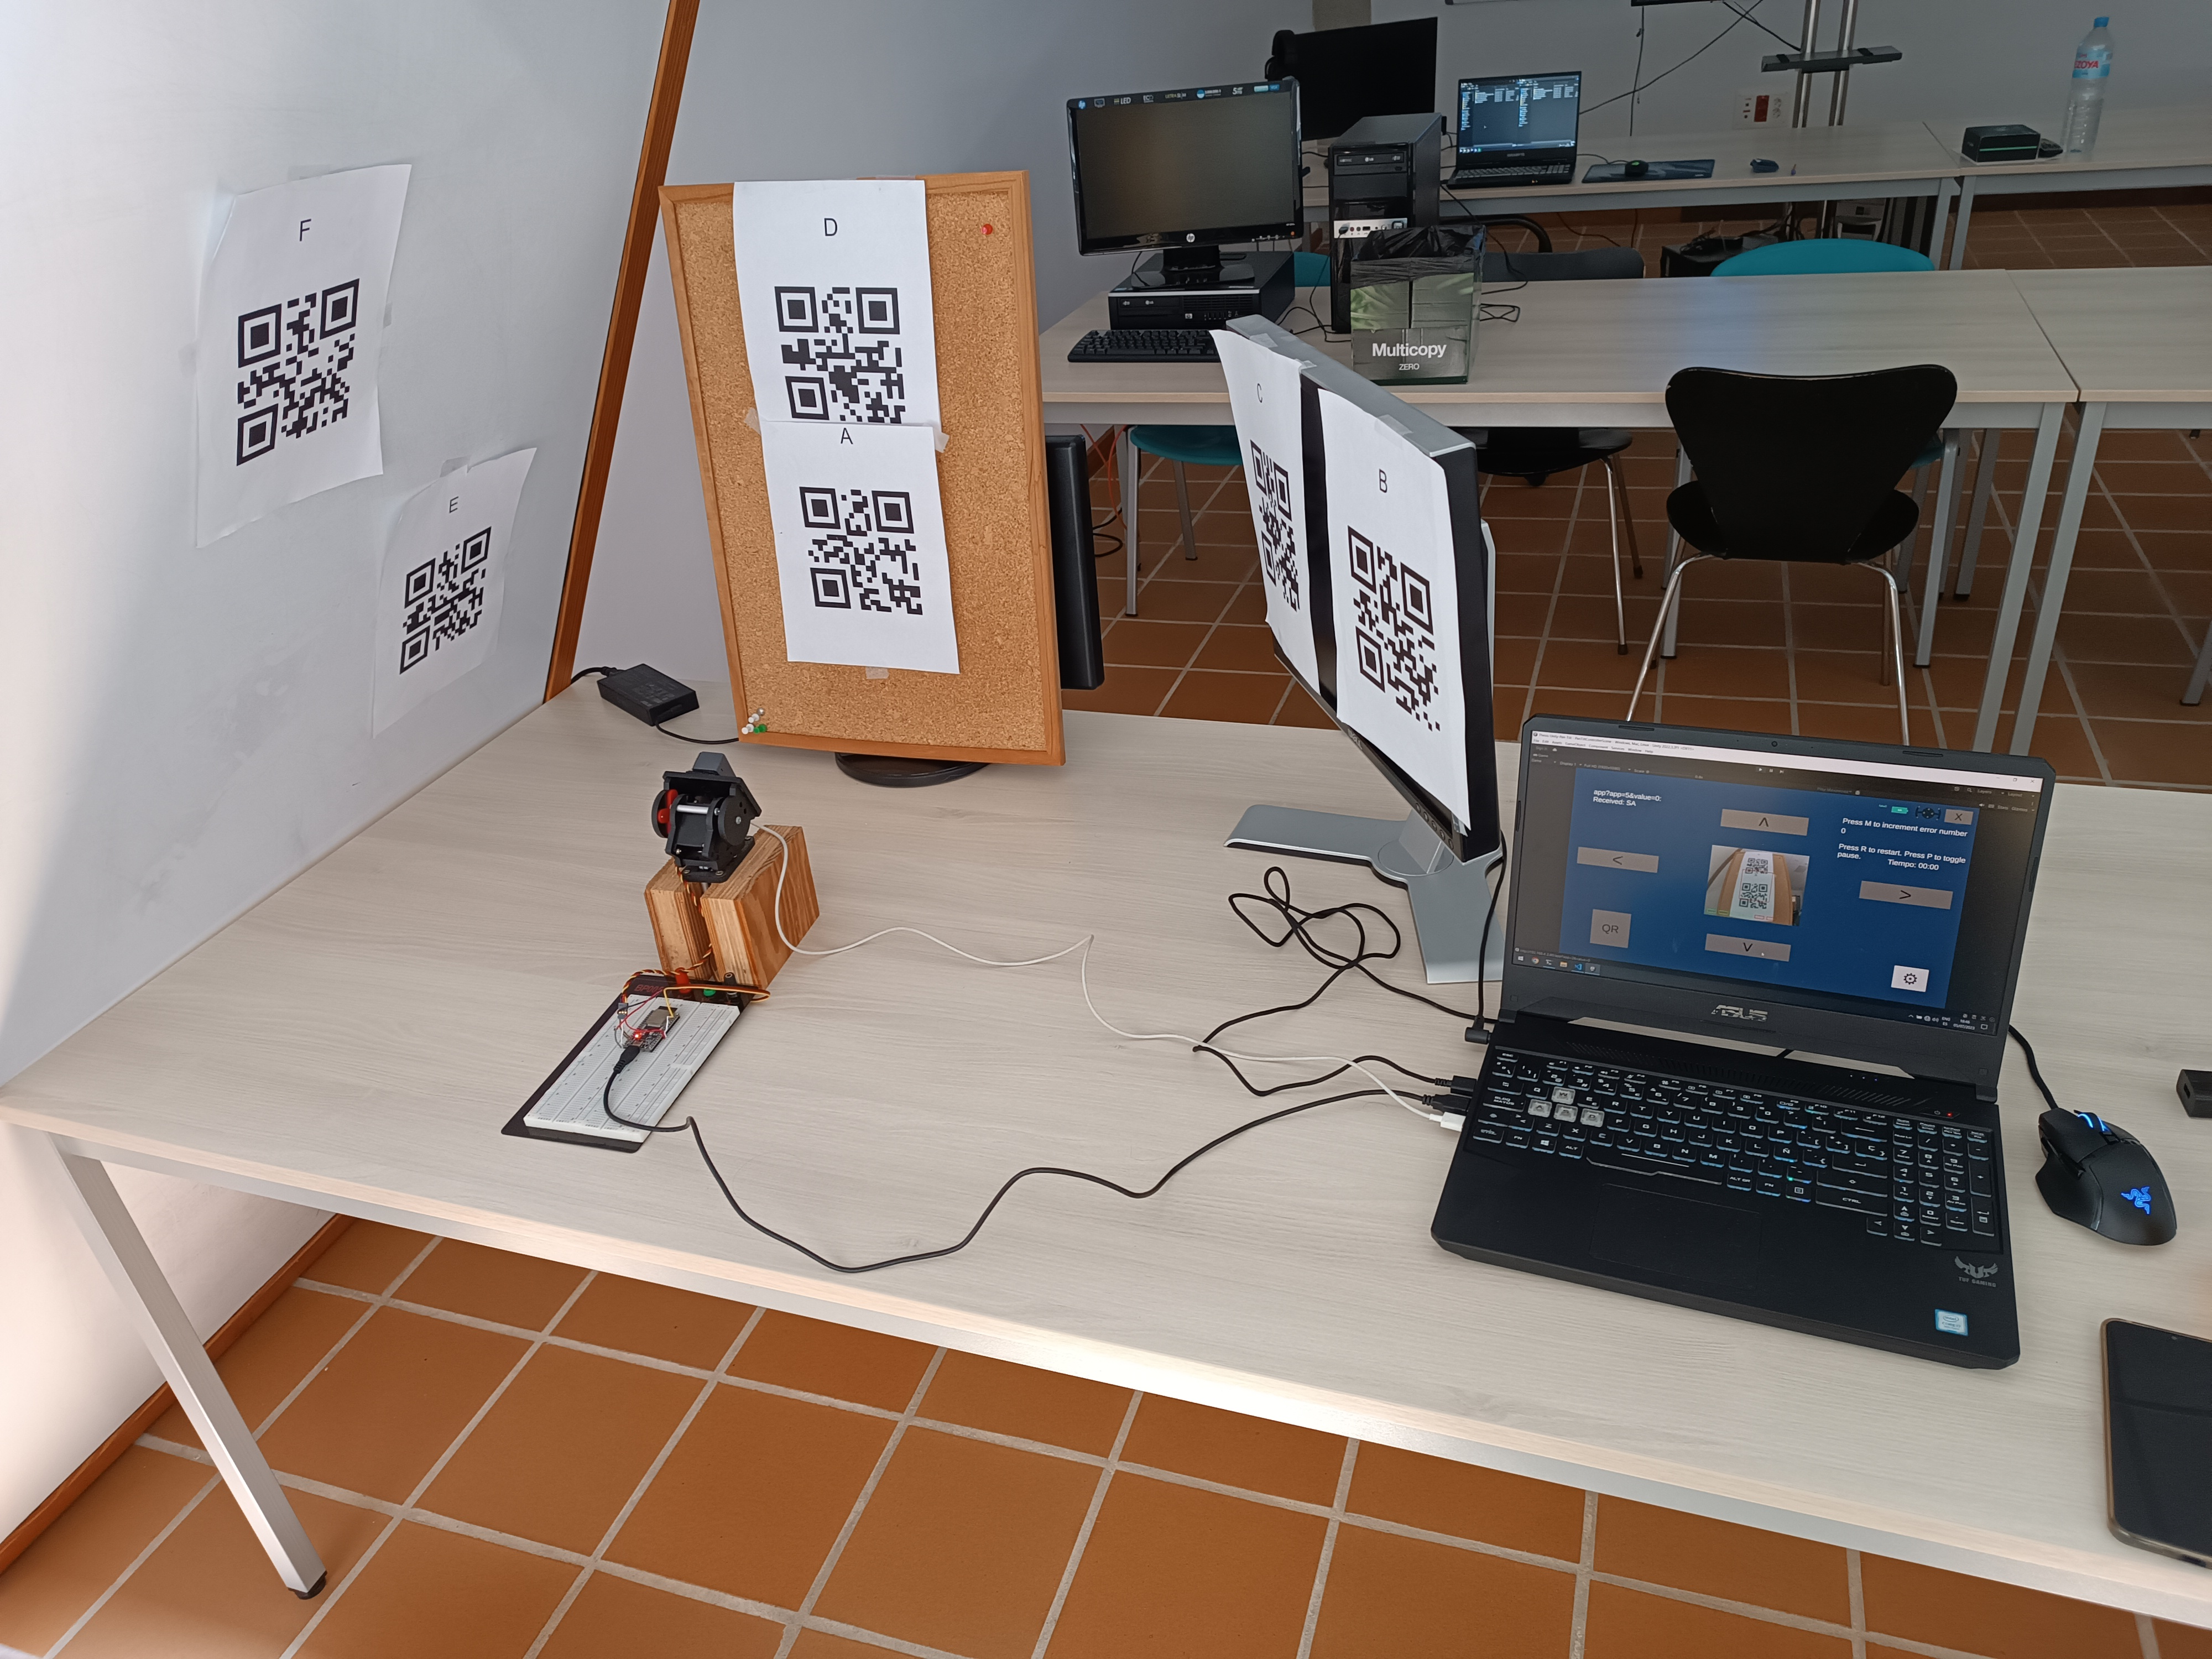
\includegraphics[width=0.7\linewidth]{figures/entorno-prueba.jpg}
   \caption{Circuito de QR}
   \label{figure:entorno-prueba}
\end{figure}

\begin{figure}[!htb]
   \centering
    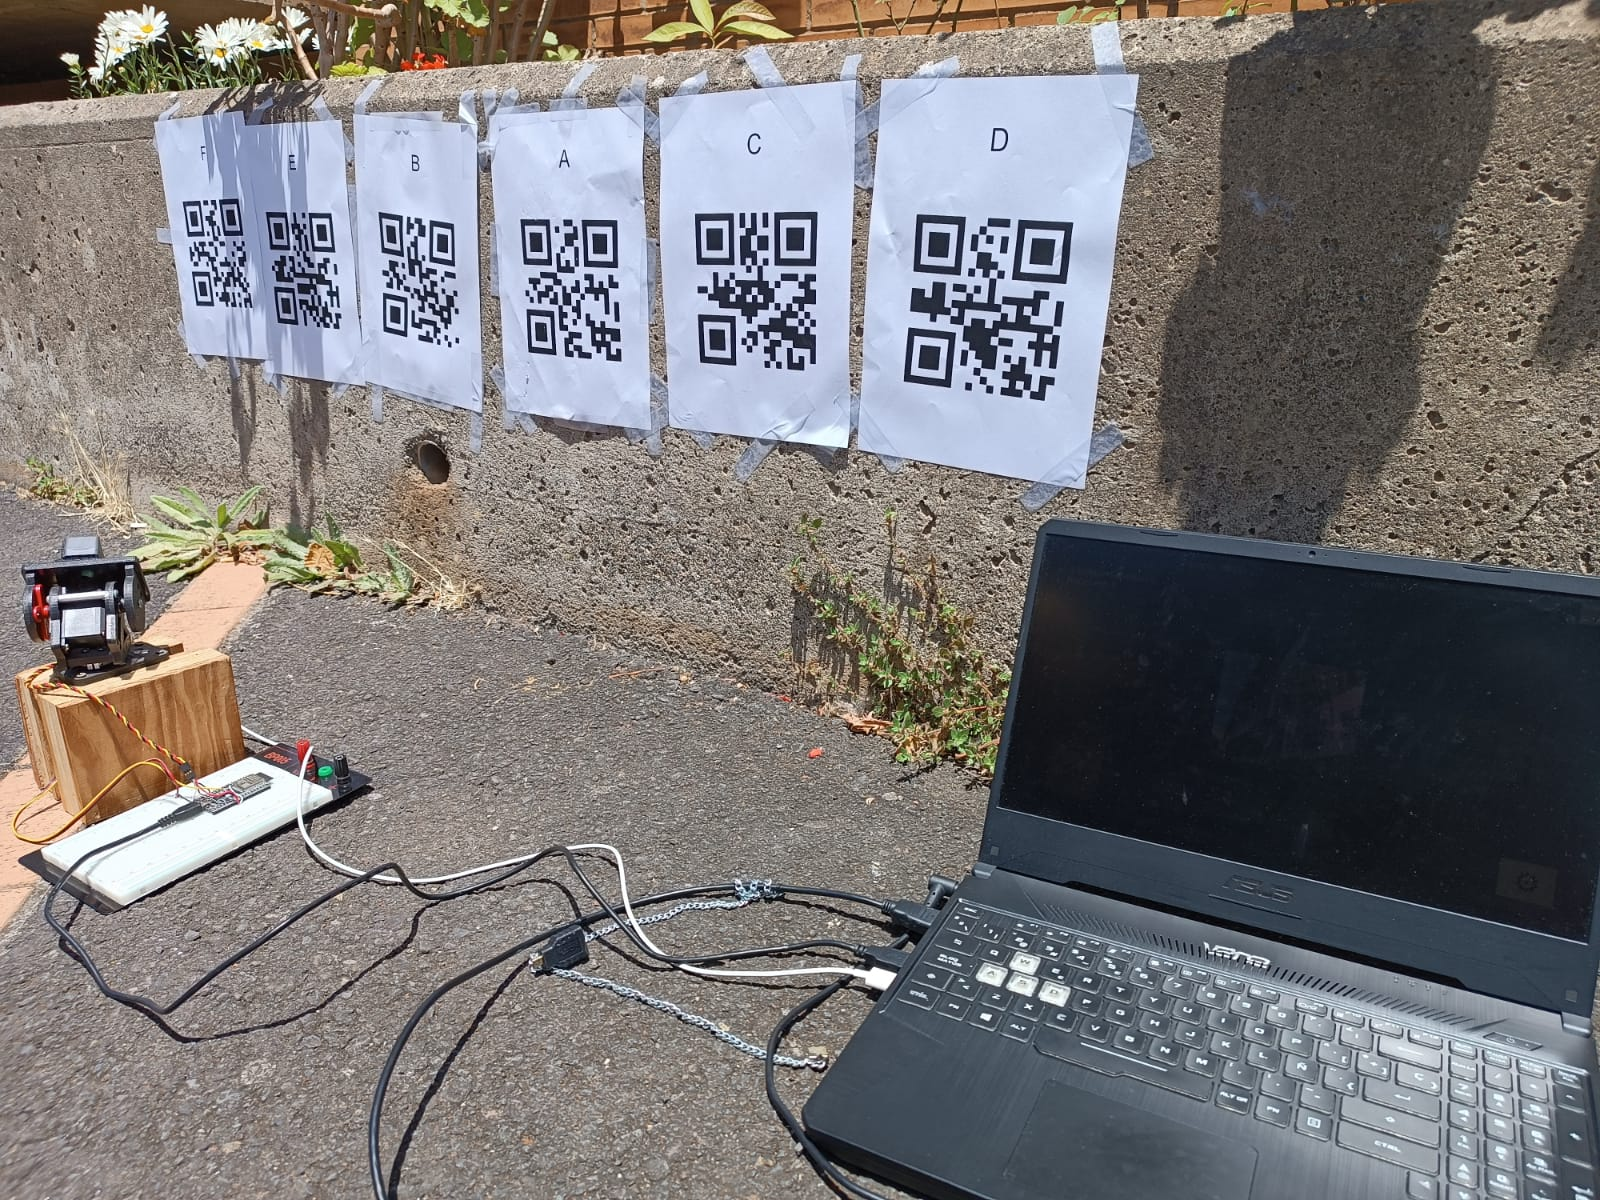
\includegraphics[width=0.7\linewidth]{figures/entorno-prueba-exterior.jpg}
   \caption{Circuito de QR en el exterior}
   \label{figure:entorno-prueba-exterior}
\end{figure}


\begin{figure}[!htb]
   \centering
    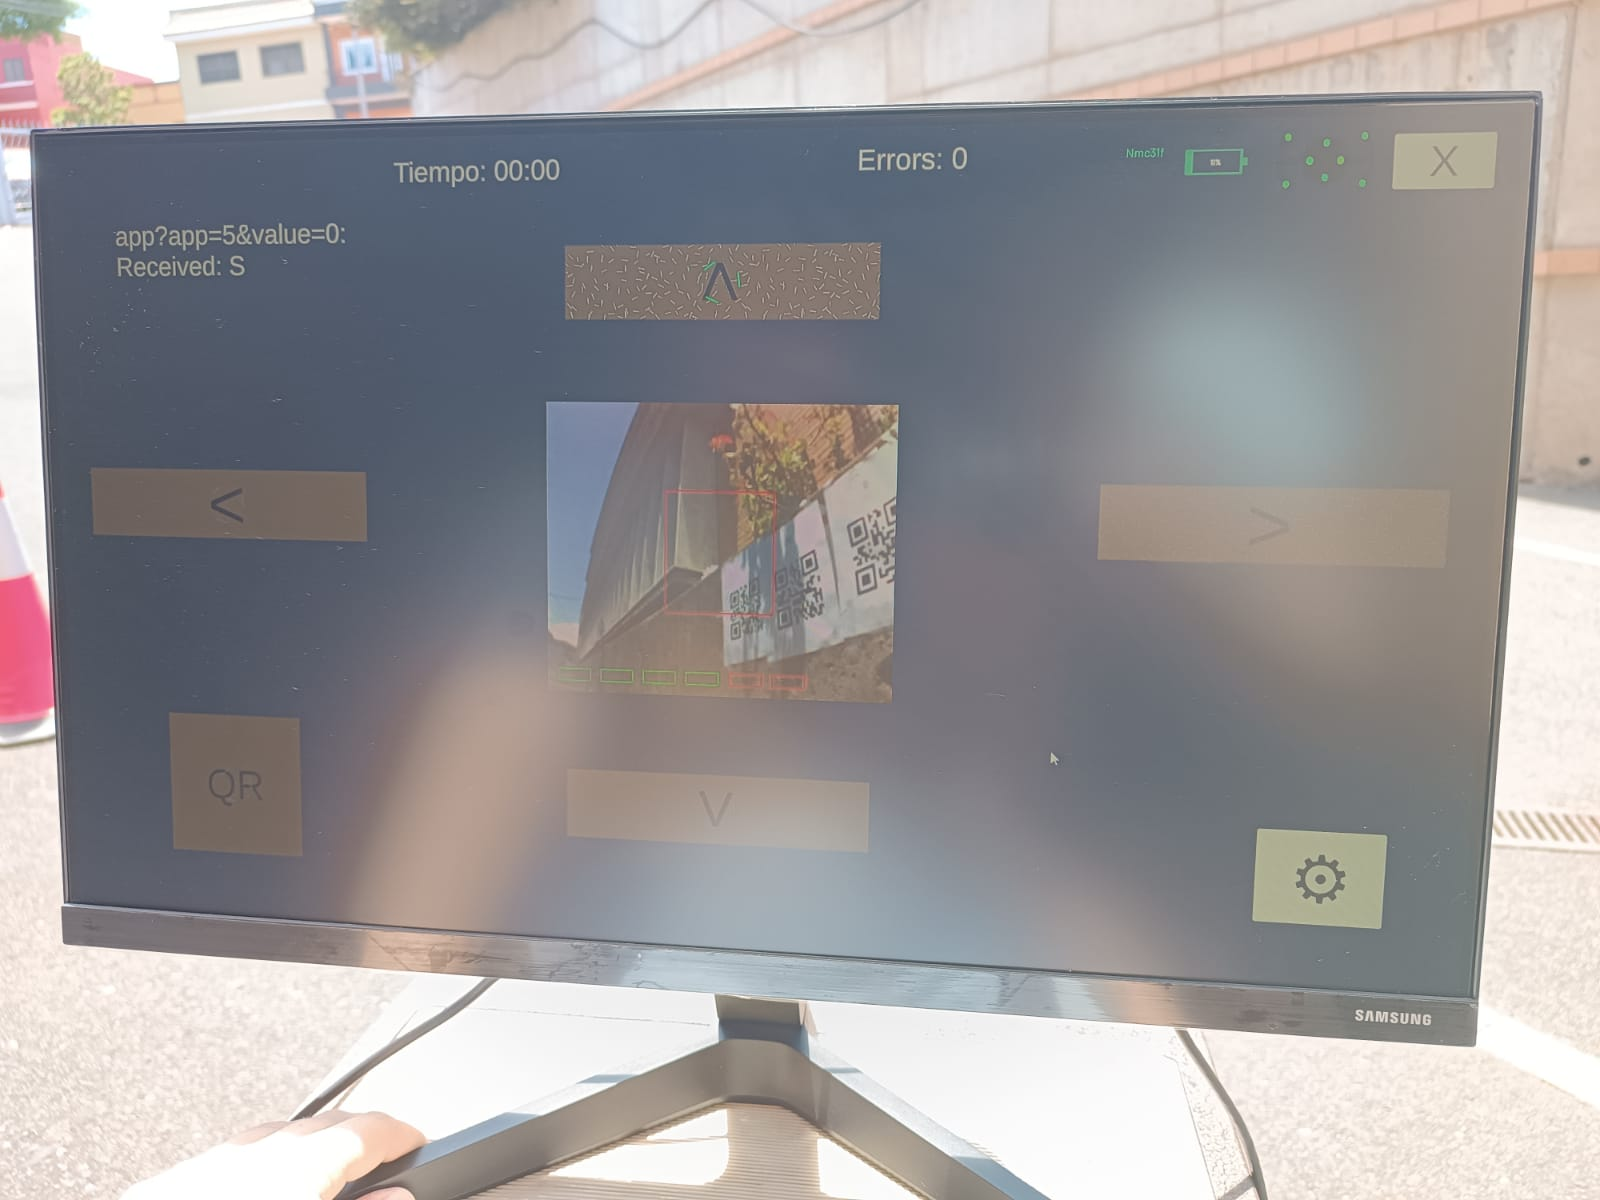
\includegraphics[width=0.6\linewidth]{figures/aplicacion-exterior.jpg}
   \caption{Prototipo Unity en el exterior}
   \label{figure:aplicacion-exterior}
\end{figure}



\section{Presentación de los datos obtenidos}
Los datos obtenidos de los 16 participantes se presentan en la tabla \ref{tab:relevantData}. Esta incluye variables como el tipo y la longitud del pelo, la nota de calibración, la luminosidad durante el uso del dispositivo y el tiempo total de uso de la interfaz cerebro-computadora (BCI).



La longitud y el tipo de pelo se recogieron debido a su potencial impacto en la capacidad del dispositivo NextMind de leer correctamente las señales cerebrales. Este aspecto es esencial para comprender las limitaciones de la interfaz en poblaciones con diferentes tipos de cabello y longitud.



Se ha dado especial importancia a la luminosidad, considerando que el estudio está orientado hacia el uso del dispositivo en exteriores. La luz ambiental podría afectar la precisión de la interfaz, posiblemente debido a los reflejos en la superficie del dispositivo o la alteración de las señales que este intenta leer.



La nota de calibración, que es una medida de cuán precisamente se ajustó el dispositivo a las necesidades individuales del usuario, se ha correlacionado con el número de errores cometidos durante el uso y el tiempo total de uso del BCI (Tiempo BCI). Esta relación es clave para evaluar el impacto de una calibración adecuada en el rendimiento del dispositivo.



El tiempo total de uso del BCI (Tiempo BCI) y el número de errores que el usuario cometió mientras utilizaba la interfaz se registraron para determinar la efectividad y la facilidad de uso del dispositivo.



Por último, se consideró si los usuarios pudieron completar las pruebas asignadas en el tiempo establecido. Si no se podía realizar la prueba, se les asignaba el tiempo máximo posible de 10 minutos, proporcionando una medida de la duración máxima de la prueba en las circunstancias más desfavorables.


\begin{table}[!htb]
\centering
\resizebox{1\textwidth}{!} {
\begin{tabular}{|c|c|c|c|c|c|c|}
\hline
\begin{tabular}[c]{@{}c@{}}Longitud\\ del\\ pelo\end{tabular} & \begin{tabular}[c]{@{}c@{}}Tipo\\ de\\ pelo\end{tabular} & \begin{tabular}[c]{@{}c@{}}Nota\\ de\\ Calibración\end{tabular} & Luminosidad & \begin{tabular}[c]{@{}c@{}}Tiempo\\ BCI\end{tabular} & \begin{tabular}[c]{@{}c@{}}Número\\ de\\ errores\end{tabular} & \begin{tabular}[c]{@{}c@{}}¿Pudo realizar la prueba?\end{tabular} \\ \hline
Mediano/Corto                                                 & Rizado                                                   & 2                                                               & Baja        & 05:50                                                & 4                                                             & Sí                                                           \\ \hline
Rapado/Calvo                                                  & Lacio                                                    & 4                                                               & Media       & 06:32                                                & 5                                                             & Sí                                                           \\ \hline
Mediano/Corto                                                 & Rizado                                                   & 3                                                               & Media       & 05:05                                                & 4                                                             & Sí                                                           \\ \hline
Rapado/Calvo                                                  & Lacio                                                    & 1                                                               & Baja        & 10:00                                                & -                                                             & No                                                           \\ \hline
Largo                                                         & Rizado                                                   & 1                                                               & Baja        & 10:00                                                & -                                                             & No                                                           \\ \hline
Rapado/Calvo                                                  & Lacio                                                    & 5                                                               & Baja        & 03:51                                                & 0                                                             & Sí                                                           \\ \hline
Largo                                                         & Lacio                                                    & 3                                                               & Baja        & 05:26                                                & 3                                                             & Sí                                                           \\ \hline
Mediano/Corto                                                 & Ondulado                                                 & 2                                                               & Media       & 10:00                                                & -                                                             & No                                                           \\ \hline
Rapado/Calvo                                                  & Lacio                                                    & 3                                                               & Media       & 07:45                                                & 2                                                             & Sí                                                           \\ \hline
Rapado/Calvo                                                  & Lacio                                                    & 2                                                               & Media       & 04:11                                                & 0                                                             & Sí                                                           \\ \hline
Largo                                                         & Rizado                                                   & 4                                                               & Media       & 03:50                                                & 0                                                             & Sí                                                           \\ \hline
Mediano/Corto                                                 & Ondulado                                                 & 5                                                               & Baja        & 02:08                                                & 0                                                             & Sí                                                           \\ \hline
Largo                                                         & Lacio                                                    & 3                                                               & Media       & 03:39                                                & 1                                                             & Sí                                                           \\ \hline
Mediano/Corto                                                 & Lacio                                                    & 3                                                               & Media       & 04:14                                                & 2                                                             & Sí                                                           \\ \hline
Mediano/Corto                                                 & Lacio                                                    & 3                                                               & Media       & 04:58                                                & 5                                                             & Sí                                                           \\ \hline
Largo                                                         & Rizado                                                   & 2                                                               & Media       & 05:19                                                & 2                                                             & Sí                                                           \\ \hline
\end{tabular}
}
\caption{Datos obtenidos en las pruebas para los 16 participantes}
\label{tab:relevantData}
\end{table}


\begin{figure}[!htb]
   \centering
    \includegraphics[width=0.7\linewidth]{figures/grafica-Calibración y Entorno de la prueba.png}
   \caption{Gráfica con la calibración y el entorno de la prueba}
   \label{figure:calibrationandtestenvironment}
\end{figure}

\begin{figure}[!htb]
   \centering
    \includegraphics[width=0.7\linewidth]{figures/grafica-Calibración y pudo realizar la prueba.png}
   \caption{Gráfica con la calibración y si pudo realizar la prueba}
   \label{figure:calibrationanddothetest}
\end{figure}

\begin{figure}[!htb]
   \centering
    \includegraphics[width=0.7\linewidth]{figures/grafica-Tiempo transcurrido y Calibración.png}
   \caption{Gráfica con el tiempo transcurrido y la calibración}
   \label{figure:timeelapsedandcalibration}
\end{figure}

\begin{figure}[!htb]
   \centering
    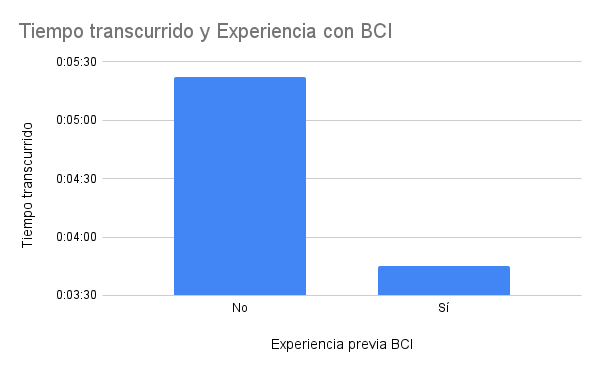
\includegraphics[width=0.7\linewidth]{figures/grafica-Tiempo transcurrido y Experiencia con BCI.png}
   \caption{Gráfica con el tiempo transcurrido y si tenía experiencia previa con el BCI}
   \label{figure:timeelapsedandpreviousexperience}
\end{figure}

\begin{figure}[!htb]
   \centering
    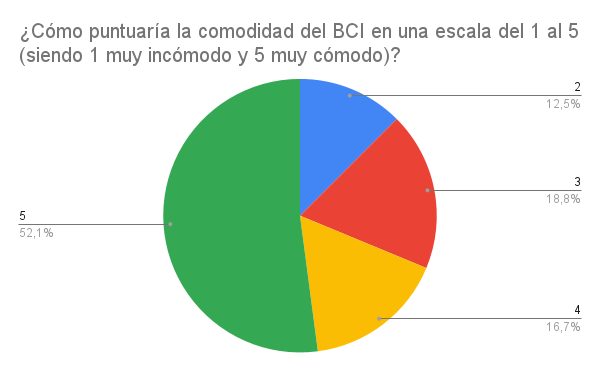
\includegraphics[width=0.7\linewidth]{figures/grafica-¿Cómo puntuaría la comodidad del BCI en una escala del 1 al 5 (siendo 1 muy incómodo y 5 muy cómodo)_.png}
   \caption{Comodidad del BCI}
   \label{figure:comfortableexperience}
\end{figure}


\section{Análisis de los datos}
A pesar de que la muestra es relativamente pequeña, se pueden extraer conclusiones significativas.



Primero, se observó que el cabello no parece influir en la calibración ni en la destreza general del BCI.



En los entornos interiores, la variación entre las calibraciones es mínima, como se puede ver en la Figura \ref{figure:calibrationandtestenvironment}.



Por otro lado, se realizaron pruebas en exteriores bajo las peores condiciones, en pleno sol a mediodía. Los resultados fueron sorprendentes. Si la persona es capaz de ver el estímulo visual (NeuroTags), el NextMind es capaz de reconocerlo sin demasiada dificultad. Se probó con el tutor, quien suele obtener un 5 en la calibración: obtuvo un 4 en la prueba y presentó tiempos de respuesta similares a los obtenidos en interiores.



El tipo de pantalla utilizada al aire libre es un factor que influye considerablemente en los resultados. Se observaron diferencias notables al utilizar pantallas más oscuras, como la mostrada en la figura \ref{figure:entorno-prueba-exterior}, en comparación con pantallas de brillo alto\ref{figure:aplicacion-exterior}. Entre las dos pantallas LCD evaluadas, la que presentaba mayor brillo incorporaba tecnología IPS, a diferencia de la otra. Además, es relevante mencionar que el brillo de las pantallas LCD puede verse afectado por la degradación con el paso del tiempo, teniendo en cuenta que ambas pantallas son LCD, una es nueva mientras que la otra tiene ya 4 años de uso, lo cual podría explicar algunas de las diferencias observadas.



La pantalla utilizada finalmente para la prueba en exterior fue un monitor SAMSUNG F24T350FHU dada por el profesorado.



Además, se encontró que cuanta más calibración se realice, más probabilidades hay de completar la prueba con éxito. Incluso con una calificación de 2, se consideró posible realizar la prueba. Solo en 1 de los 16 casos, la prueba no se pudo realizar con una calibración de 2. Ver Figura \ref{figure:calibrationanddothetest}.



Se observa una correlación aparente entre el tiempo de realización de la prueba y la calificación de calibración: a mayor calificación, menor tiempo necesario para completar la prueba (Figura \ref{figure:timeelapsedandcalibration}).



Es relevante señalar que si los participantes tienen experiencia previa con el uso de BCI, tienden a completar la prueba en menos tiempo (Figura \ref{figure:timeelapsedandpreviousexperience}).



Incluso durante la prueba, se observó una mejora continua en los participantes, independientemente de si su calificación de calibración inicial no era de 4 o 5.



También se consultó a los usuarios sobre su percepción de la comodidad del BCI. Como se aprecia en el gráfico \ref{figure:comfortableexperience}, la mayoría de los usuarios, más del 50\%, calificaron su experiencia como ``Muy cómoda'', asignándole un 5, el puntaje máximo. En contraste, solo un pequeño grupo, el 12,5\%, le dio un 2, señalando una experiencia de comodidad reducida. Es importante resaltar que ningún usuario otorgó la puntuación mínima de 1, que representaría una experiencia ``Muy incómoda''.

\section{Adaptación a un nuevo sistema}

La aplicación de Unity ha sido eficientemente adaptada a un nuevo dispositivo: un robot móvil. Este proceso ha puesto de relieve la notable adaptabilidad de la aplicación. Esta capacidad quedó patente cuando logramos recrear una nueva interfaz desde cero, reutilizando los scripts y prefabs existentes, en un plazo de menos de dos horas.



El entorno donde se llevó a cabo esta prueba se puede observar en la figura \ref{figure:entorno-prueba-robot}.

\begin{figure}[!htb]
   \centering
    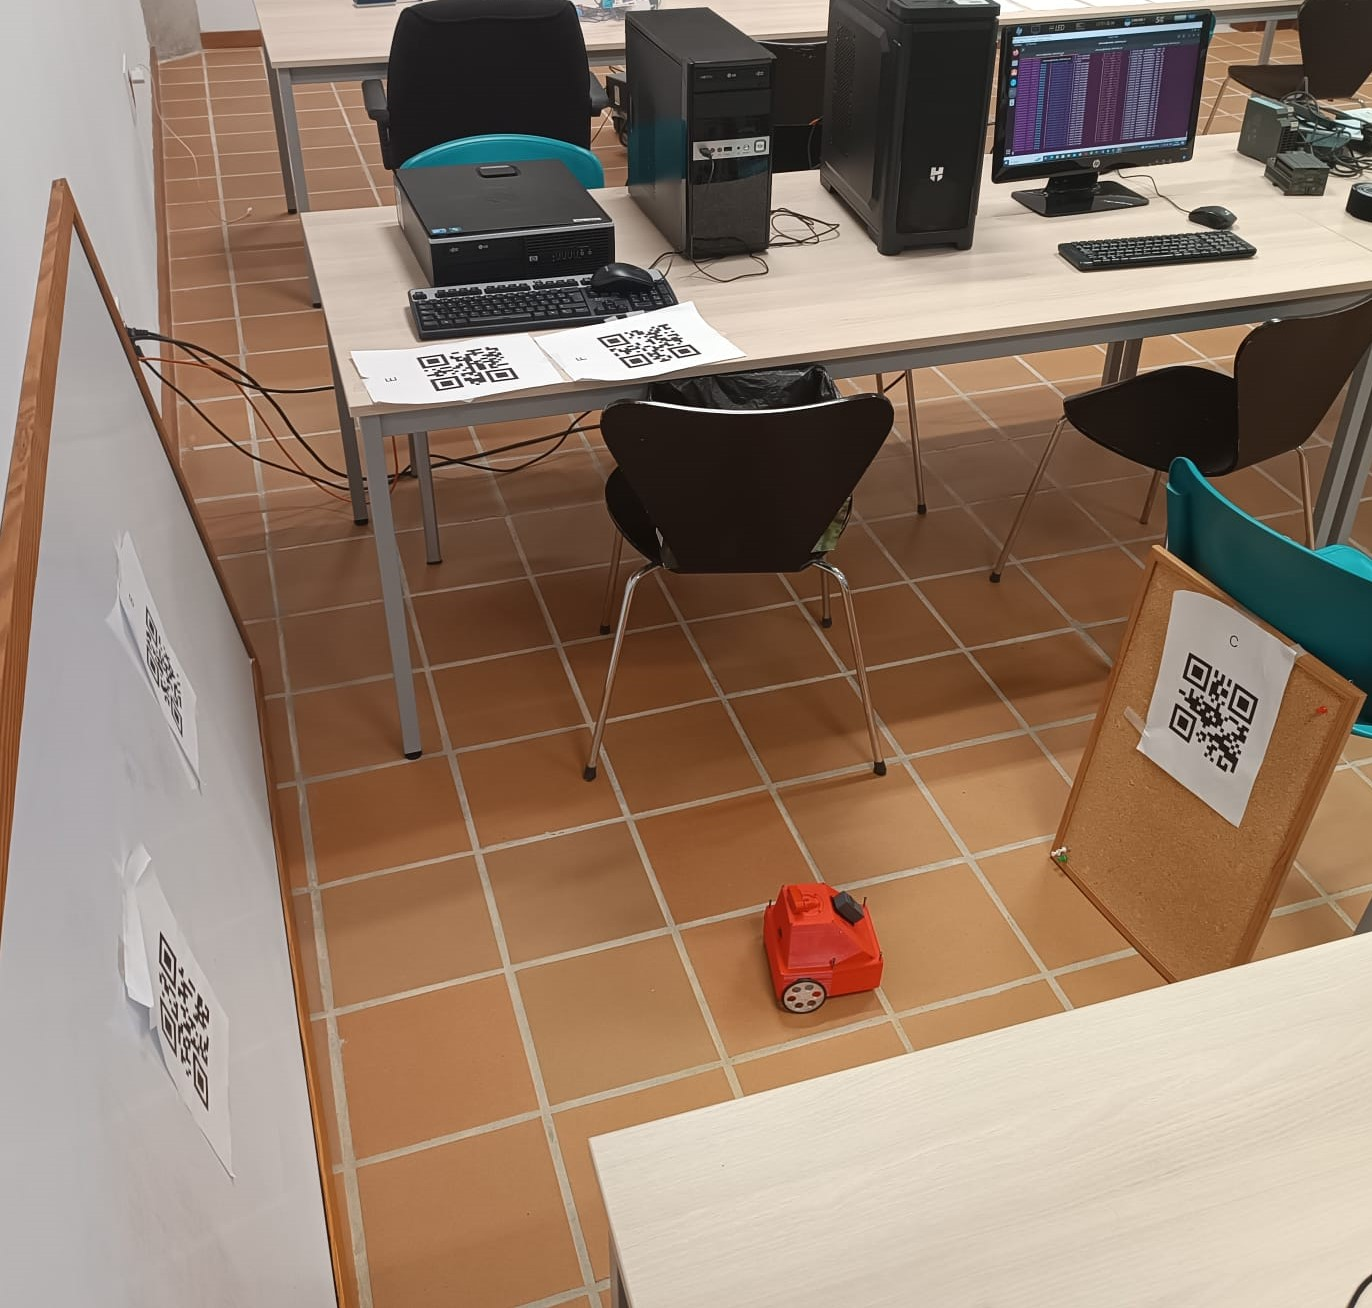
\includegraphics[width=0.6\linewidth]{figures/entorno-prueba-robot.jpg}
   \caption{Entorno de la prueba del robot}
   \label{figure:entorno-prueba-robot}
\end{figure}


\section{Conclusiones}

Este estudio revela la efectividad y versatilidad de NextMind en diversas condiciones y contextos. El dispositivo NextMind demuestra ser un BCI accesible para una amplia variedad de usuarios, sin ser afectado por factores como la presencia de cabello. Muestra una robustez considerable, funcionando de manera efectiva tanto en ambientes interiores como exteriores. Adicionalmente, el rendimiento del dispositivo parece ser casi inmune a las variaciones de luz ambiental, lo cual es un hallazgo que puede orientar el desarrollo futuro de dispositivos BCI. Además, la eficiencia de NextMind tiende a mejorar con una calibración de mayor precisión y con la experiencia previa con dispositivos BCI, lo que destaca la importancia de familiarizarse con esta tecnología. En términos de comodidad, más del 50\% de los usuarios encontraron que NextMind era ``Muy cómodo'', lo que sugiere una alta aceptabilidad y potencial para su uso continuado.



Para concluir, la interfaz ha demostrado una notable capacidad para adaptarse a diversos contextos y sistemas. Esta flexibilidad refuerza su utilidad, al permitir que se aplique de manera efectiva en una amplia gama de situaciones, haciendo que la interfaz sea una herramienta versátil y eficiente en el campo de la robótica.

